\section{Real systems in enlarged regions}\label{app:enlarged}

To test whether the gain grows on real systems as $p$ decreases, we enlarged the region of initial conditions by a factor of $k$ about its center, $B_k=kB$ with $k=2$--16, keeping the escape radius at least twice the distance to the farthest corner of the region. If the basin lay inside $B$, its measure in $B_k$ would be $p_{k=1}/k^3$. It is not (Table~\ref{tab:enlarged}, Figure~\ref{fig:enlarged}a): for SE11, $p$ falls from $7.7\times10^{-3}$ only to $2.4\times10^{-4}$ at $k=16$, against the expected $1.9\times10^{-6}$, and the other systems behave similarly. The basins of these hidden attractors extend far beyond $B$, so their rarity is a property of the chosen region rather than of the attractor. Continuation of the hidden attractors in a parameter gives the same conclusion: in Chua~II and in the Wang--Chen and Wei systems, the basin fraction stays within $10^{-3}$--$0.7$ up to the crisis at which the attractor disappears, and in LE1, it falls at most to $2.4\times10^{-4}$. Over the enlarged regions, the gain grows as $p$ decreases on three of the five systems (Figure~\ref{fig:enlarged}b): on SE11, from 3.1 to 24; on LE1, from 6.2 to 16; and on Chua~I, from 1.2 to 6.3. The effective growth exponents, i.e., the slopes of $\ln G$ against $\ln(1/p)$, are 0.3--0.6, with the caveat that the enlargement changes the geometry of the basin as well as its measure. On Chua~II, the gain of the portfolio falls from 7.4 to 0.71 at $k=4$, and splitting alone falls to 0.14, because the longest transients belong to trajectories that return slowly from far away rather than to the neighborhood of the target. On the Jafari cycle, where there is no signal, the portfolio stays at 0.24--0.43, within the guarantee.

\begin{table}[tbhp]
\centering
\caption{Real systems in the enlarged regions $kB$ ($R=50$; $k=1$: $R=100$): basin measure, cost of uniform sampling, and gains $G_{0.9}$ with 95\% bootstrap intervals. Bold: values whose lower interval bound exceeds 1; a lower bound of 0 means that some bootstrap resamples did not reach 90\% success; ``---'' with a percentage: fewer than 90\% of the runs found the target.}
\label{tab:enlarged}
\footnotesize
\setlength{\tabcolsep}{3pt}

\begin{tabular}{lrrrrr}
\toprule
System & $k$ & $p$ & $N^0_{0.9}$ & Splitting & Portfolio \\
\midrule
SE11 & 1 & 0.0077 & 317 & \textbf{2.53} \ci{1.95}{2.86} & \textbf{3.10} \ci{2.46}{3.70} \\
SE11 & 2 & 0.0023 & 811 & \textbf{3.91} \ci{3.03}{4.66} & \textbf{4.93} \ci{3.96}{6.01} \\
SE11 & 4 & $6.1\times10^{-4}$ & 3858 & \textbf{11.8} \ci{6.38}{19.4} & \textbf{17.5} \ci{8.95}{26.8} \\
SE11 & 8 & $4.5\times10^{-4}$ & 5191 & \textbf{9.92} \ci{5.54}{14.5} & \textbf{9.19} \ci{5.87}{17.0} \\
SE11 & 16 & $2.4\times10^{-4}$ & 9351 & \textbf{15.8} \ci{9.96}{21.8} & \textbf{24.2} \ci{13.8}{34.5} \\
LE1 & 1 & 0.0013 & 1617 & \textbf{8.29} \ci{6.35}{12.3} & \textbf{6.24} \ci{3.76}{10.0} \\
LE1 & 2 & $5.3\times10^{-4}$ & 4540 & \textbf{8.81} \ci{6.08}{17.2} & \textbf{7.51} \ci{2.41}{14.4} \\
LE1 & 4 & $3.4\times10^{-4}$ & 5911 & \textbf{11.1} \ci{7.35}{23.5} & \textbf{7.19} \ci{2.99}{10.5} \\
LE1 & 8 & $1.8\times10^{-4}$ & 13\,229 & \textbf{18.3} \ci{12.9}{27.9} & \textbf{15.9} \ci{10.8}{23.0} \\
Chua I & 1 & 0.033 & 66 & 1.20 \ci{0.92}{1.77} & 1.24 \ci{0.94}{1.77} \\
Chua I & 2 & 0.0083 & 267 & \textbf{2.30} \ci{1.61}{3.23} & \textbf{2.61} \ci{1.87}{3.84} \\
Chua I & 4 & 0.0010 & 2230 & \textbf{6.48} \ci{3.32}{10.7} & \textbf{5.58} \ci{3.80}{9.62} \\
Chua I & 8 & $1.8\times10^{-4}$ & 11\,169 & \textbf{6.16} \ci{4.16}{12.5} & \textbf{6.30} \ci{4.04}{13.9} \\
Chua II & 1 & 0.0026 & 818 & \textbf{5.05} \ci{4.13}{7.07} & \textbf{7.36} \ci{6.09}{10.2} \\
Chua II & 2 & $7.7\times10^{-4}$ & 2891 & \textbf{2.61} \ci{1.71}{4.11} & \textbf{3.74} \ci{2.67}{7.55} \\
Chua II & 4 & $2.1\times10^{-4}$ & 8988 & 0.14 \ci{0.10}{0.25} & 0.71 \ci{0.57}{1.36} \\
Jafari cycle & 1 & 0.010 & 219 & 0.29 \ci{0.19}{0.53} & 0.43 \ci{0.29}{0.78} \\
Jafari cycle & 2 & 0.0016 & 1245 & 0.22 \ci{0}{0.30} & 0.34 \ci{0}{0.57} \\
Jafari cycle & 4 & $2.2\times10^{-4}$ & 10\,061 & --- (88\%) & 0.24 \ci{0}{0.35} \\
\bottomrule
\end{tabular}

\end{table}

\begin{figure}[tbhp]
\centering
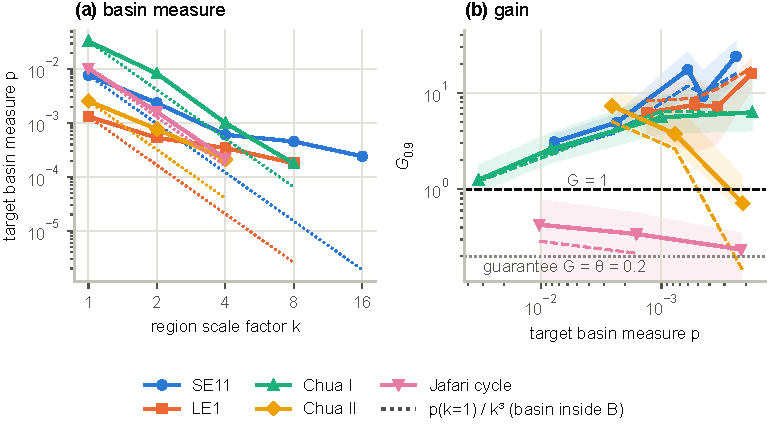
\includegraphics[width=\textwidth]{figures/fig27_enlarged_regions.pdf}
\caption{Real systems in enlarged regions $kB$. (a) Basin measure of the hidden target versus $k$; dotted lines: $p_{k=1}/k^3$, the measure if the basin lay inside $B$. (b) Gain of the portfolio (solid, with 95\% intervals) and of splitting (dashed) versus the basin measure, which decreases to the right. Dashed horizontal line: $G=1$; dotted: the guarantee $G=\theta=0.2$.}
\label{fig:enlarged}
\end{figure}

